\section{Research Support}

\begin{frame}{Research and Data Science Services}
\begin{itemize}
  \item Provide research computing support, consultations, and collaborations
  \item Data Science - Dr. Eric Godat
  \item High-Performance Computing - Dr. Robert Kalescky \& Dr. John LaGrone
  \item Custom Devices (IOT, wearables, etc.) - Guillermo Vasquez
\end{itemize}
\end{frame}

\begin{frame}{Center for Research Computing (CRC)}
\begin{itemize}
  \item Maintains our primary shared resource for research computing, ManeFrame II (M2), in collaboration with OIT
  \item Provides research computing tools, support, and training to all faculty, staff, and students using research computing resources
  \item \url{www.smu.edu/crc} has documentation and news
  \item \href{mailto:help@smu.edu}{help@smu.edu} or \href{mailto:rkalescky@smu.edu}{rkalescky@smu.edu} for help
  \item Request an account at \url{www.smu.edu/crc}
\end{itemize}
\end{frame}

\begin{frame}{Spring 2022 CRC HPC Workshop Series}
\begin{table}
\tiny
\begin{tabular}{lll}
Date     & Time  & Workshop\\
\hline
February 2 & 2-4 & ManeFrame II (M2) Introduction \\  
February 9 & 2-4 & Workflows in R \\  
February 15 & 3-5 & Finding and Preparing Text Data Sets for Mining \\
Febryary 16 & 1-4 & Machine Learning with Python Part 1 \\
February 17 & 12-1 & AI for the Non-Expert \\
February 18 & 12-1 & Introduction to GitHub \\        
February 23 & 2-4  & Containers and Spack \\     
March 2   &  2-4 &  ManeFrame II (M2) Introduction \\
March 3   &  1-4 & Data Science Workflow with R \\  
March 8   &  3-6 & Introduction to Python for Text Mining \\ 
March 9   &  1-4 & Machine Learning with Python Part 2 \\ 
March 22  &  3-6 & Getting Support for Text Mining \\  
March 23  &  2-4 & Shared Memory Parallelism \\   
March 30  &  1-4 & Deep Learning with Python Part 1 \\   
April 6   &  2-4 & ManeFrame II (M2) Introduction \\    
April 13  &  2-4 & Accelerator Libraries and APIs \\    
April 20  &  1-4 & Deep Learning with Python Part 2 \\      
April 27  &  2-4 & MPI/NCCL/SHMem \\            
May 4     &  2-4 & ManeFrame II (M2) Introduction      
\end{tabular}
\caption{Workshops will be held each Wednesday from 2:00 to 4:00 PM. Sessions will typically be                                
recorded and posted along with session materials.         
Register on the Library Workshop Calendar \href{https://libcal.smu.edu/calendar/libraryworkshops}{https://libcal.smu.edu/calendar/libraryworkshops}
}
\end{table}
\end{frame}

\section{ManeFrame II (M2)}

\begin{frame}{Cluster Super Computers}
\begin{figure}
  \centering
  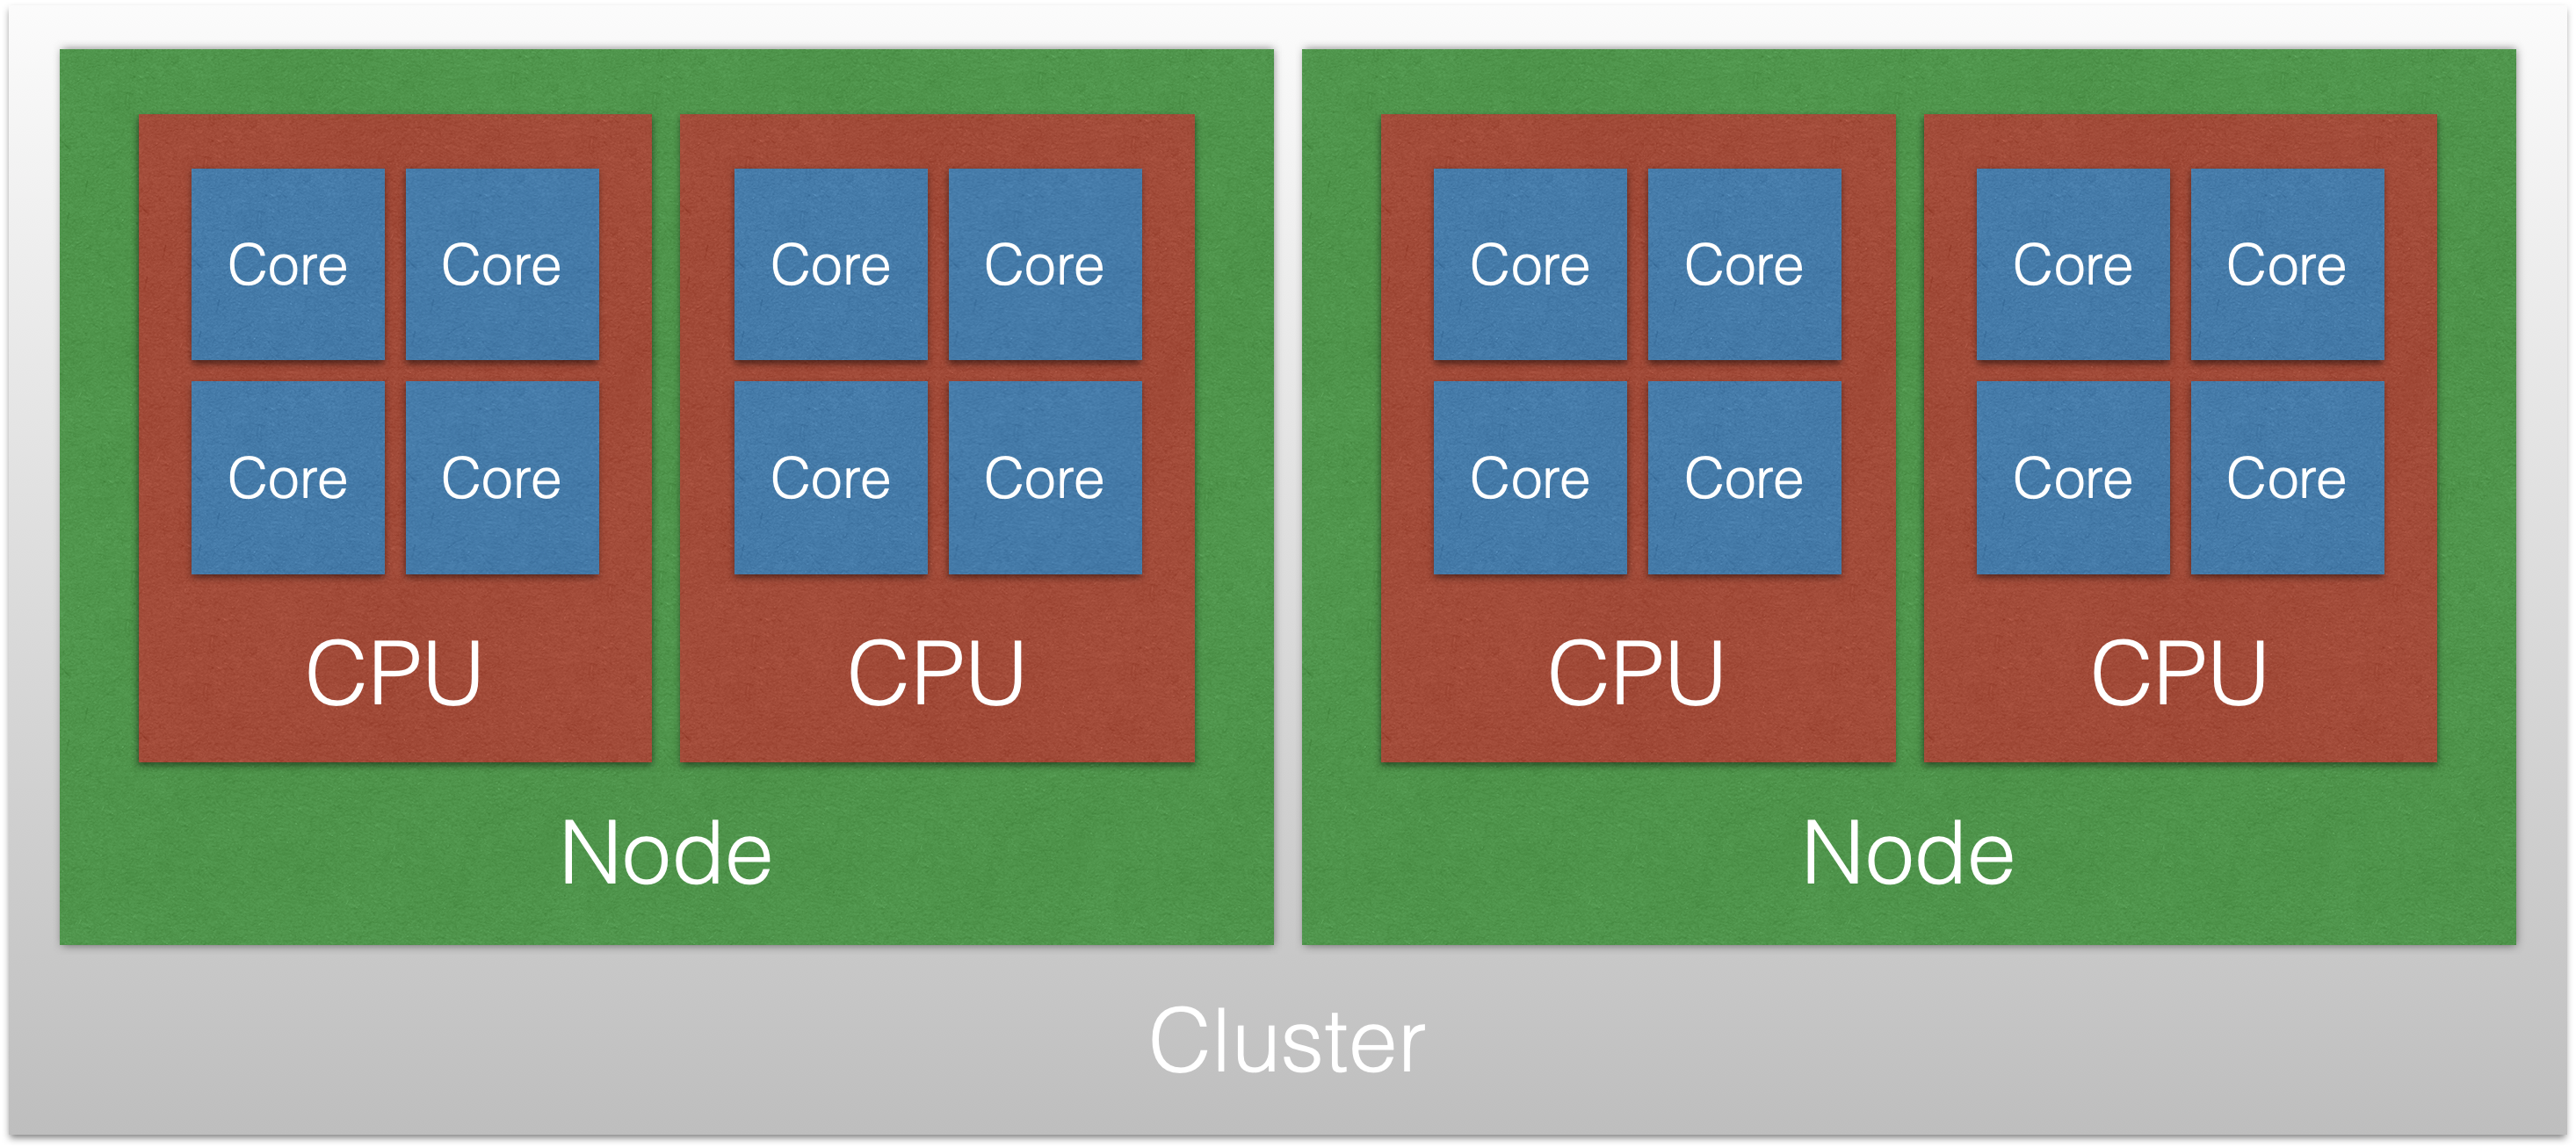
\includegraphics[width=0.75\linewidth]{figures/cluster.png}
  \caption{A cluster is a collection of individual computers networked together. Applications can be configured to run on all available compute resources.}
\end{figure}
\end{frame}

\begin{frame}{ManeFrame II (M2) Node Types}
\begin{table}
\tiny
\begin{tabular}{lllll}
\toprule
Type & Quantity & Cores & Memory [GB] & Additional Resources\\
\midrule
Standard-Memory & 176 & 36 & 256 & \\
Medium-Memory-1 & 35 & 36 & 768 & \\
Medium-Memory-2 & 4 & 24 & 768 & 3 TB SSD local scratch\\
High-Memory-1 & 5 & 36 & 1,536 & \\
High-Memory-2 & 6 & 40 & 1,536 & 3 TB SSD local scratch\\
GPGPU-1 & 36 & 36 & 256 & NVIDIA P100 GPU has 3,584 CUDA cores and 16 GB CoWoS\\
MIC-1 & 36 & 64 & 384 & 16 GB of high bandwidth (400 GB/s) stacked memory\\
VDI & 5 & 36 & 256 & NVIDIA Quadro M5000 GPU\\
v100x8 & 3 & 36 & 768 & 8 NVIDIA V100 GPUs with 5,120 CUDA cores and 32 GB CoWoS\\
Faculty Partner Nodes & 3 &  &  & Various research specific NVIDIA GPU configurations\\
\midrule
ManeFrame II & 354 & 11,276 & 120 TB & 2.8 PB storage and InfiniBand network\\
\bottomrule
\end{tabular}
\end{table}
\end{frame}

\begin{frame}{ManeFrame II (M2) Partitions (Queues)}
\begin{table}
\tiny
\begin{tabular}{llll}
\toprule
Partition & Duration & Cores & Memory [GB]\\
\midrule
development & 2 hours & various & various\\
htc & 1 day & 1 & 6\\
standard-mem-s & 1 day & 36 & 256\\
standard-mem-m & 1 week & 36 & 256\\
standard-mem-l & 1 month & 36 & 256\\
medium-mem-1-s & 1 day & 36 & 768\\
medium-mem-1-m & 1 week & 36 & 768\\
medium-mem-1-l & 1 month & 36 & 768\\
medium-mem-2 & 2 weeks & 24 & 768\\
high-mem-1 & 2 weeks & 36 & 1538\\
high-mem-2 & 2 weeks & 40 & 1538\\
mic & 1 week & 64 & 384\\
gpgpu-1 & 1 week & 36 & 256\\
v100x8 & 1 week & 1 & 20\\
fp-gpgpu-2 & various & 24 & 128\\
fp-gpgpu-3 & various & 40 & 384\\
\bottomrule
\end{tabular}
\end{table}
\end{frame}

\begin{frame}{ManeFrame II File Systems}
\begin{description}
\item[\$HOME]
\begin{itemize}
  \item Default file system when logging into M2, e.g. \mintinline{sh}{/users/$USER}.
  \item Space should be used to write, edit, compile programs, and job submission scripts, etc.
  \item Restricted by quotas (200 GB) and backed-up.
\end{itemize}
\item[\$WORK]
\begin{itemize}
  \item Long term storage at \mintinline{sh}{/work/users/$USER}.
  \item Restricted by quotas (8 TB) and not backed-up.
\end{itemize}
\item[\$SCRATCH]
\begin{itemize}
 \item Scratch space at \mintinline{sh}{/scratch/users/$USER}.
 \item Treat \$SCRATCH as a volatile file system that is not backed-up.
 \item Beginning October 1, 2021, \mintinline{sh}{$SCRATCH} has a 60-day retention policy, i.e. untouched files will be removed after 60 days.
\end{itemize}
\end{description}
\end{frame}

